\documentclass[conference]{IEEEtran}

% ======================================================================
% PREAMBLE
% ======================================================================

% ----------------------------------------------------------------------
% Page layout
% ----------------------------------------------------------------------
\usepackage[a4paper,margin=25mm]{geometry}

% ----------------------------------------------------------------------
% Tables and floats
% ----------------------------------------------------------------------
\usepackage{booktabs,tabularx,array}
\usepackage{textcomp} % for \textdegree
\newcolumntype{L}[1]{>{\raggedright\arraybackslash}p{#1}}
\usepackage{float} % Table placement: use [H]
\usepackage{subcaption} % Subfigures / subcaptions
\usepackage{graphicx}
\graphicspath{{figures/}}
\usepackage{rotating}

% ----------------------------------------------------------------------
% Colors
% ----------------------------------------------------------------------
\usepackage{xcolor}
\definecolor{LinkBlue}{HTML}{1F4E79}

% ----------------------------------------------------------------------
% Fonts and math
% ----------------------------------------------------------------------
\usepackage[T1]{fontenc}
\usepackage{textcomp}

% IBM Plex Sans as main document font
\usepackage[sfdefault,scale=0.95]{plex-sans}
\renewcommand{\familydefault}{\sfdefault}

% IBM Plex Mono for monospace text
\usepackage[scale=0.95]{plex-mono}

% Section headings without small caps
% Section headings without small caps
\makeatletter
\renewcommand\section{\@startsection{section}{1}{\z@}%
  {-1.4ex \@plus -0.4ex \@minus -.2ex}%
  {1.4ex \@plus .2ex}%
  {\normalfont\sffamily\large\bfseries\centering}}

\renewcommand\subsection{\@startsection{subsection}{2}{\z@}%
  {-1.5ex \@plus -0.5ex \@minus -.2ex}%
  {0.8ex \@plus .2ex}%
  {\normalfont\sffamily\normalsize\bfseries}}

\renewcommand\subsubsection{\@startsection{subsubsection}{3}{\z@}%
  {-1.5ex \@plus -0.5ex \@minus -.2ex}%
  {0.8ex \@plus .2ex}%
  {\normalfont\sffamily\normalsize\bfseries}}
\makeatother

% Math
\usepackage{amsmath,amssymb}
\usepackage[upint]{newtxsf}

% ----------------------------------------------------------------------
% Units
% ----------------------------------------------------------------------
\usepackage{siunitx}
\sisetup{detect-all=true}

% ----------------------------------------------------------------------
% Bibliography
% ----------------------------------------------------------------------
\usepackage[backend=biber,style=numeric,sorting=none]{biblatex}
\addbibresource{references.bib}

% ----------------------------------------------------------------------
% Hyperlinks
% ----------------------------------------------------------------------
\usepackage[hypertexnames=false]{hyperref}
\hypersetup{
    colorlinks=true,
    linkcolor=black,
    citecolor=black,
    urlcolor=LinkBlue
}
\urlstyle{same}
\usepackage{fontawesome5}

% ======================================================================
% TITLE / AUTHOR METADATA
% ======================================================================
\newcommand{\ReportRepositoryURL}{https://github.com/MarcosVerdejoBosch/Discrete-Linear-Regulator}
\newcommand{\ReportRepositoryText}{GitHub repo}

\title{Linear Voltage Regulator}

\author{
\IEEEauthorblockN{Marcos Verdejo Bosch}
\IEEEauthorblockA{
\faGithub\ \href{\ReportRepositoryURL}{\ReportRepositoryText}
}
}

% ======================================================================
% DOCUMENT START
% ======================================================================
\begin{document}

\maketitle

\begin{abstract}
This work presents a largely discrete linear regulator built around a PNP pass element with selectable 5\,V and 3.3\,V outputs. The design includes output regulation, current limiting, undervoltage lockout, and overvoltage lockout. Its architecture and circuit implementation are described, and nominal regulation, transient response, protection operation, and regulation-loop stability are evaluated in LTspice. A PCB was designed, fabricated, and assembled, with initial checks confirming both output settings. Detailed hardware characterization remains pending; the simulated results provide reference values for these measurements.
\end{abstract}

% ======================================================================
% OVERVIEW AND THEORY
% ======================================================================

\section{Introduction}

\subsection{Overview}

\noindent A voltage regulator supplies a load with a stable dc voltage. Many circuits require such regulation because supply variations and noise can affect their operation. The main building blocks of a linear regulator are the series pass element, the feedback network, the reference voltage, and the error amplifier. The pass element is placed between the input and the output so that the regulator can control the current delivered to the load. The feedback network senses the output voltage, and the error amplifier compares it with the reference voltage. The resulting error signal drives the pass element, keeping the output voltage near its target value as input and load conditions vary. \cite{razavi_ldo_2019}

Figure~\ref{fig:block_diagram} shows a functional diagram of this linear regulator. The divider \(R_1\)-\(R_2\) samples \(V_{out}\) and generates the feedback voltage \(V_{fb}\). The error amplifier uses the difference between \(V_{fb}\) and \(V_{ref}\) as the control error for the pass element. If \(V_{fb}\) moves away from \(V_{ref}\), the amplifier changes the pass-element drive until this error is reduced. This action regulates \(V_{out}\). \cite{ti_linear_switching_fundamentals}

\begin{figure}[H]
    \centering
    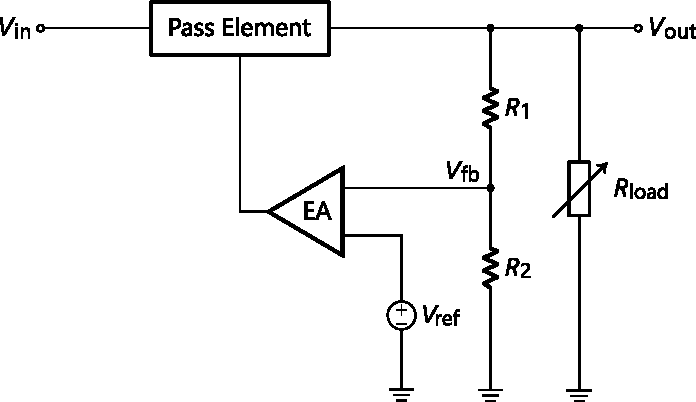
\includegraphics[width=\columnwidth]{blockdiagram.pdf}
    \caption{Functional diagram of the linear regulator.}
    \label{fig:block_diagram}
\end{figure}

For the resistive feedback divider,
\[
V_{fb}=V_{out}\frac{R_2}{R_1+R_2}.
\]

In normal operation, the loop adjusts the pass element until \(V_{fb} \approx V_{ref}\). Substituting this condition gives
\[
V_{out}\approx V_{ref}\left(1+\frac{R_1}{R_2}\right).
\]

Thus, \(V_{out}\) is set by the reference voltage and the feedback-divider ratio. \cite{razavi_ldo_2019}

The regulator presented in this work follows this feedback principle using a largely discrete implementation with a PNP pass element. The following sections describe its design objectives, main features, and architecture.

\subsection{Design Objectives}

The main objective of this work is to obtain a regulated output in both selectable modes while supporting load currents up to 1\,A. The design is evaluated under line and load variations to verify static regulation and transient behavior.

A second objective is to make the main protection functions measurable. Undervoltage lockout, overvoltage lockout, and short-circuit current limiting are characterized in simulation and used as reference points for prototype validation.

\subsection{Key Features}

Table~\ref{tab:key_features} summarizes the main features of the proposed regulator.

\begin{table}[H]
\centering
\footnotesize
\setlength{\tabcolsep}{4pt}
\begin{tabularx}{\columnwidth}{@{}L{3.0cm}X@{}}
\toprule
\textbf{Feature} & \textbf{Value} \\
\midrule
Topology & Largely discrete linear regulator \\
Pass element & PNP transistor \\
Output voltage & 5\,V / 3.3\,V selectable \\
Output current & 1\,A design target; evaluated in simulation \\
Current limit & Approximately 1.5\,A nominal setting \\
Input protection & UVLO / OVLO \\
Prototype & PCB-based hardware prototype \\
\bottomrule
\end{tabularx}
\caption{Key features of the proposed regulator.}
\label{tab:key_features}
\end{table}

\section{Regulator Architecture}

\subsection{Architecture Overview}

The proposed regulator combines a PNP series pass transistor, a voltage-feedback loop, selectable output voltage, and protection circuits. Figure~\ref{fig:regulator_architecture} shows the functional arrangement of these blocks. The switches, protection circuits, and reference source are simplified representations of the circuits described in the next section.

\begin{figure}[H]
    \centering
    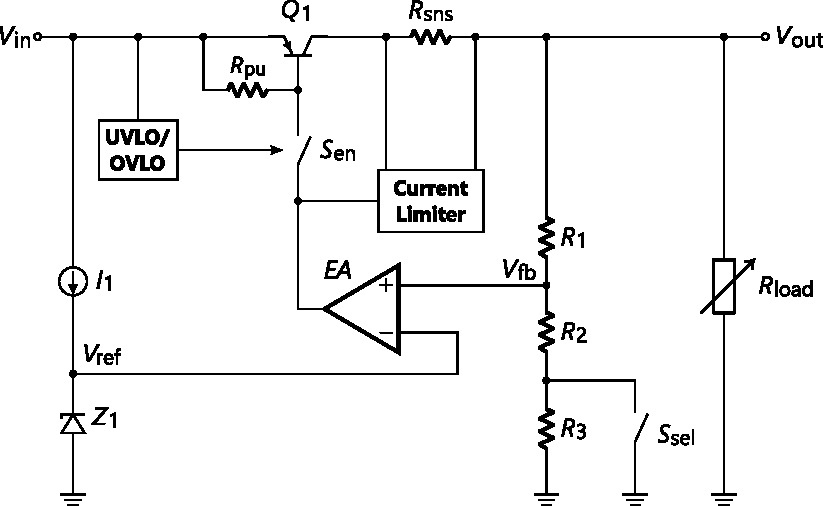
\includegraphics[width=\columnwidth]{architecture.pdf}
    \caption{Functional schematic of the proposed linear regulator.}
    \label{fig:regulator_architecture}
\end{figure}

The PNP pass transistor \(Q_1\) supplies the load through the current-sense resistor \(R_{\mathrm{sns}}\). The feedback divider senses the output voltage after this resistor and supplies \(V_{\mathrm{fb}}\) to the error amplifier, which controls the pass transistor by comparing \(V_{\mathrm{fb}}\) with \(V_{\mathrm{ref}}\). The reference branch is represented by the current source \(I_1\) and the shunt reference \(Z_1\). Output-voltage selection is performed by \(S_{\mathrm{sel}}\), which bypasses \(R_3\) to change the feedback ratio between the 5\,V and 3.3\,V settings.

The protection functions act on the pass-transistor drive. The current limiter senses the voltage across \(R_{\mathrm{sns}}\) and modifies the drive when the current threshold is reached. The UVLO/OVLO block controls the enable switch \(S_{\mathrm{en}}\), disconnecting the drive path when the input voltage is outside the permitted range. With this switch open, \(R_{\mathrm{pu}}\) pulls the base of \(Q_1\) toward its emitter to turn the pass transistor off.

% ======================================================================
% CIRCUIT IMPLEMENTATION
% ======================================================================
\section{Circuit Implementation}

The architecture shown in Fig.~\ref{fig:regulator_architecture}
is implemented using a largely discrete regulation stage
together with integrated reference, operational-amplifier,
and comparator circuits. Figure~\ref{fig:circuit_schematic}
presents the complete schematic.

The following discussion focuses on the error amplifier
and its interface with the PNP pass transistor, which form
the core of the voltage-regulation loop. An annotated
detail of this stage is provided in
Fig.~\ref{fig:error_amplifier_detail} to identify its
functional blocks and support the explanation of the
main design choices. The reference, output-selection,
enable, and protection circuits are described in the
subsequent subsections using the complete schematic.

\begin{sidewaysfigure*}
    \centering
    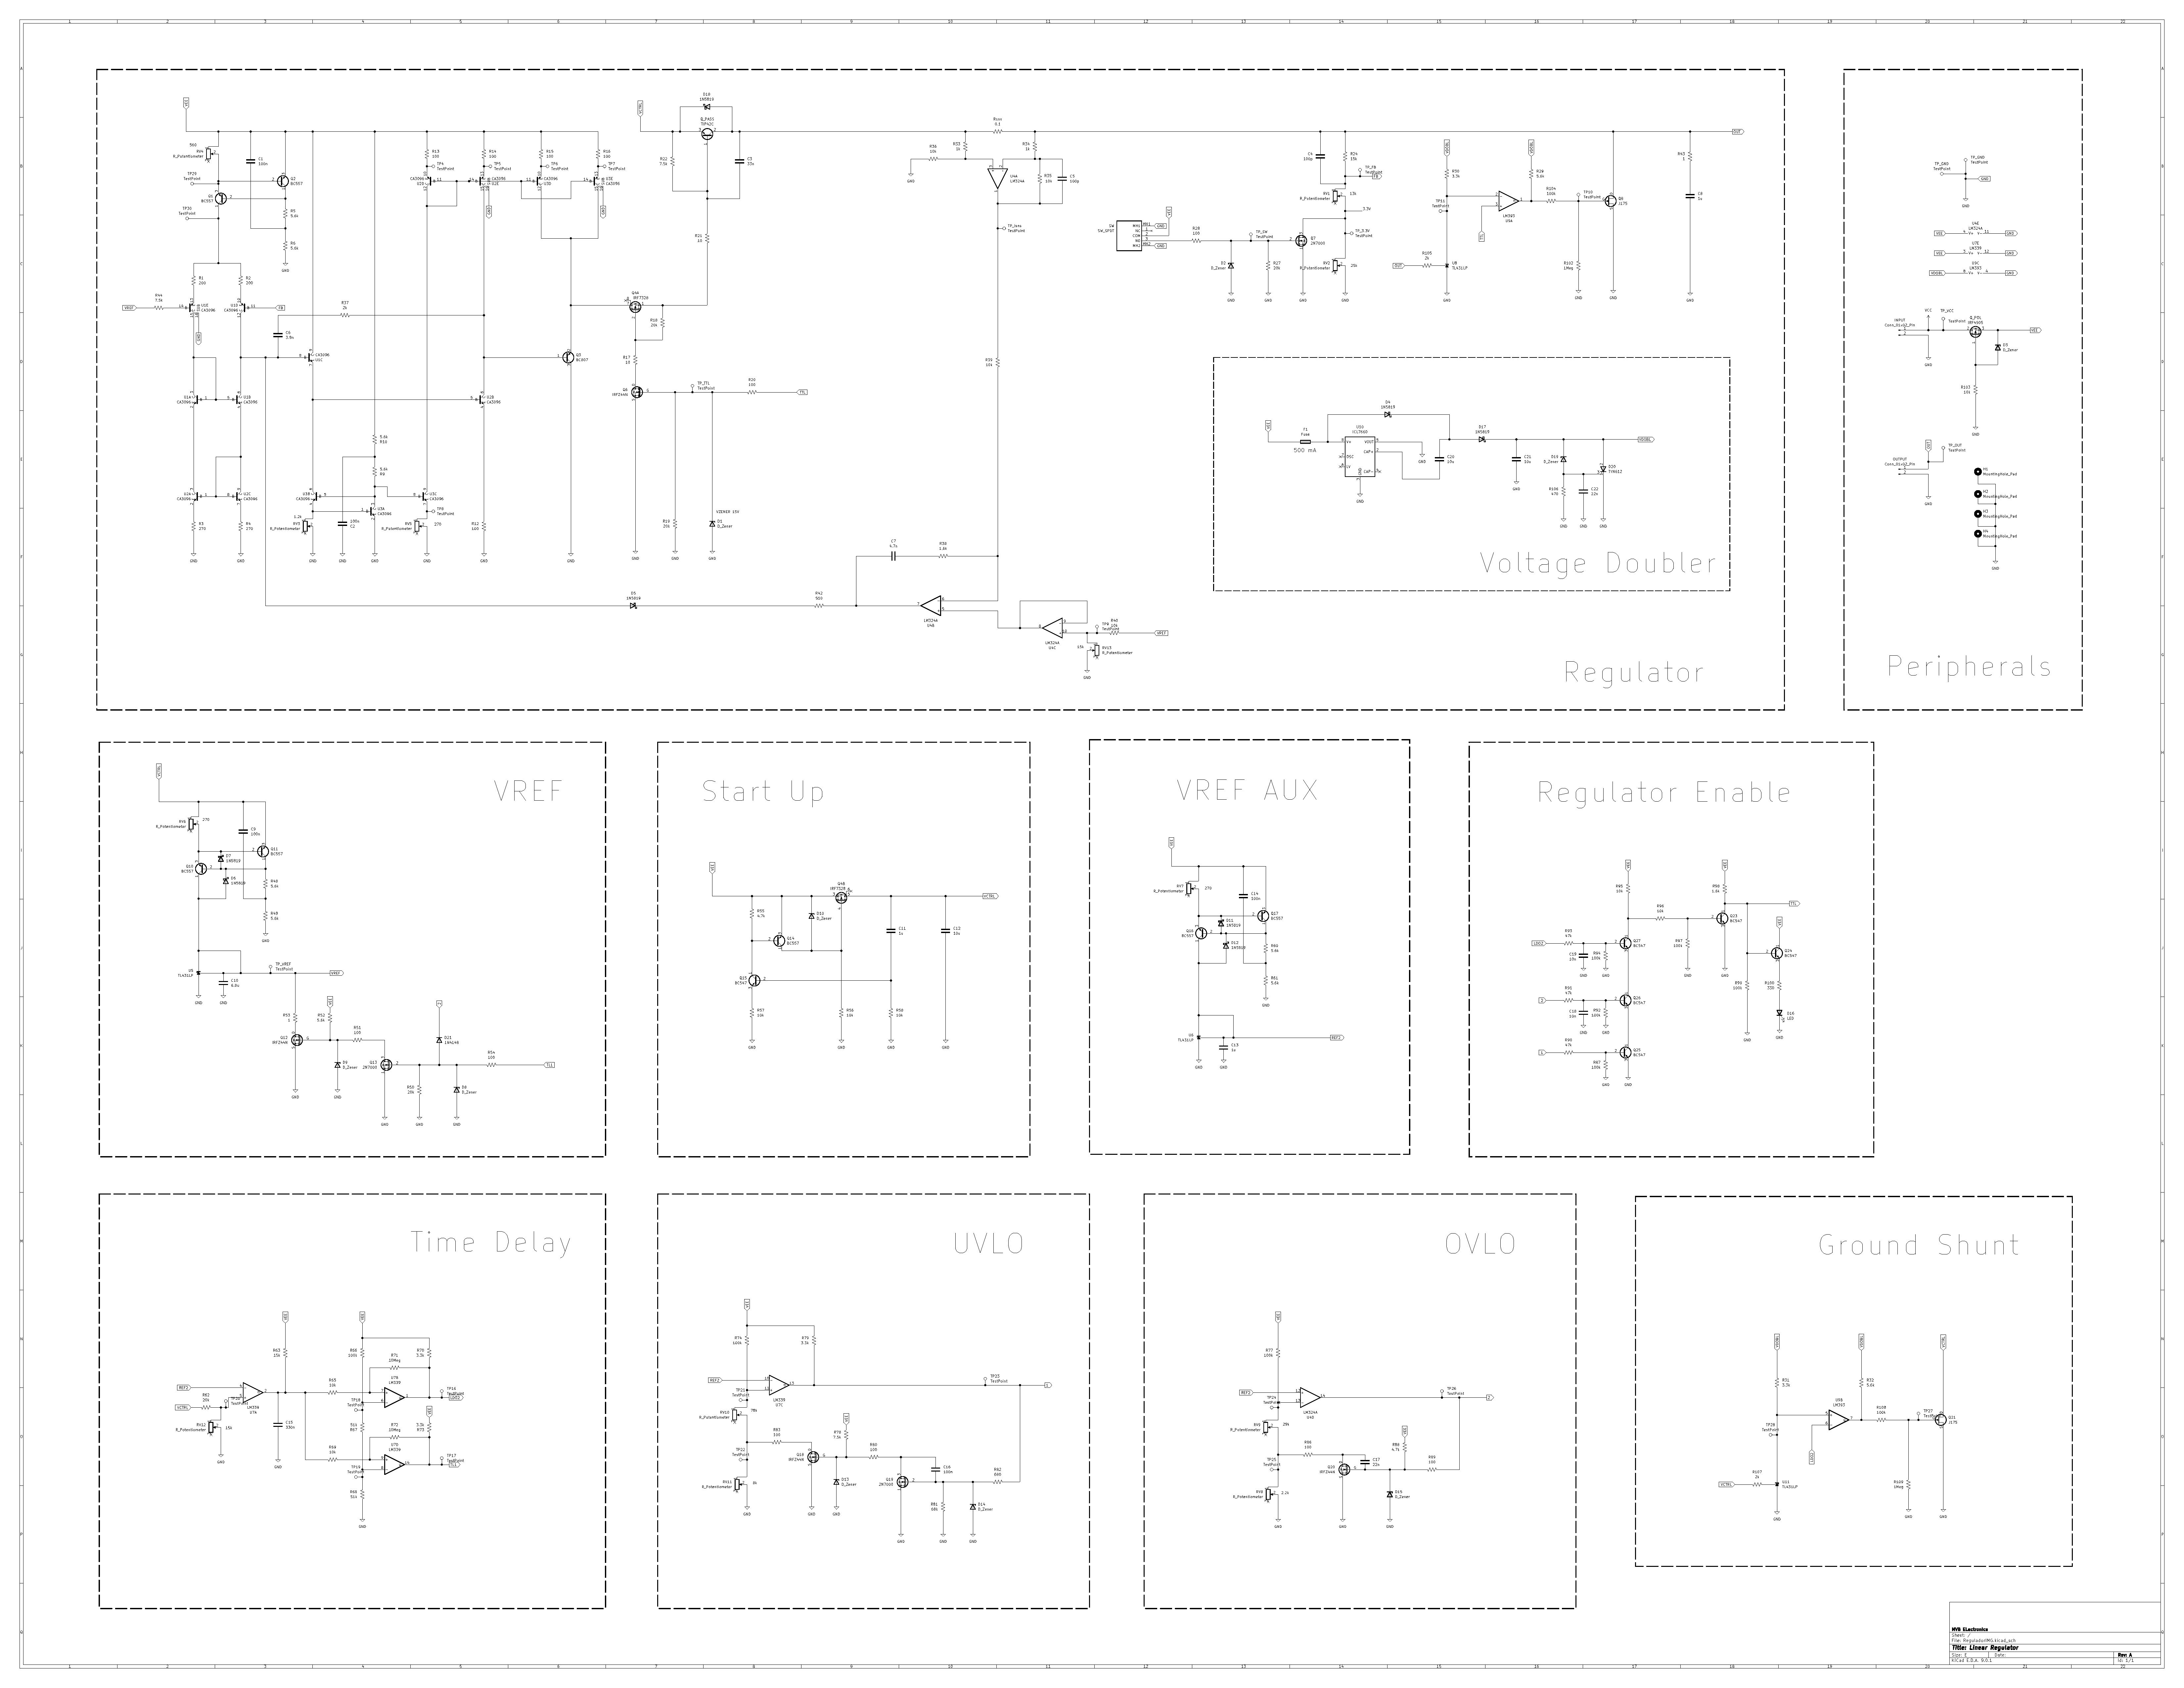
\includegraphics[width=\textheight]{ReguladorIMG.pdf}
    \caption{Complete circuit schematic of the proposed
    linear regulator.}
    \label{fig:circuit_schematic}
\end{sidewaysfigure*}

\subsection{Regulation Stage}

Figure~\ref{fig:error_amplifier_detail} shows an annotated
detail of the regulation stage. The error amplifier compares
the feedback voltage \(V_{\mathrm{fb}}\) with the reference
\(V_{\mathrm{ref}}\) and controls the PNP pass transistor
\(Q_{\mathrm{pass}}\). Its implementation comprises a
differential input stage, a voltage-amplification stage
(VAS) with an emitter-follower input, and a Class-A
output stage.

\begin{figure*}[t]
    \centering
    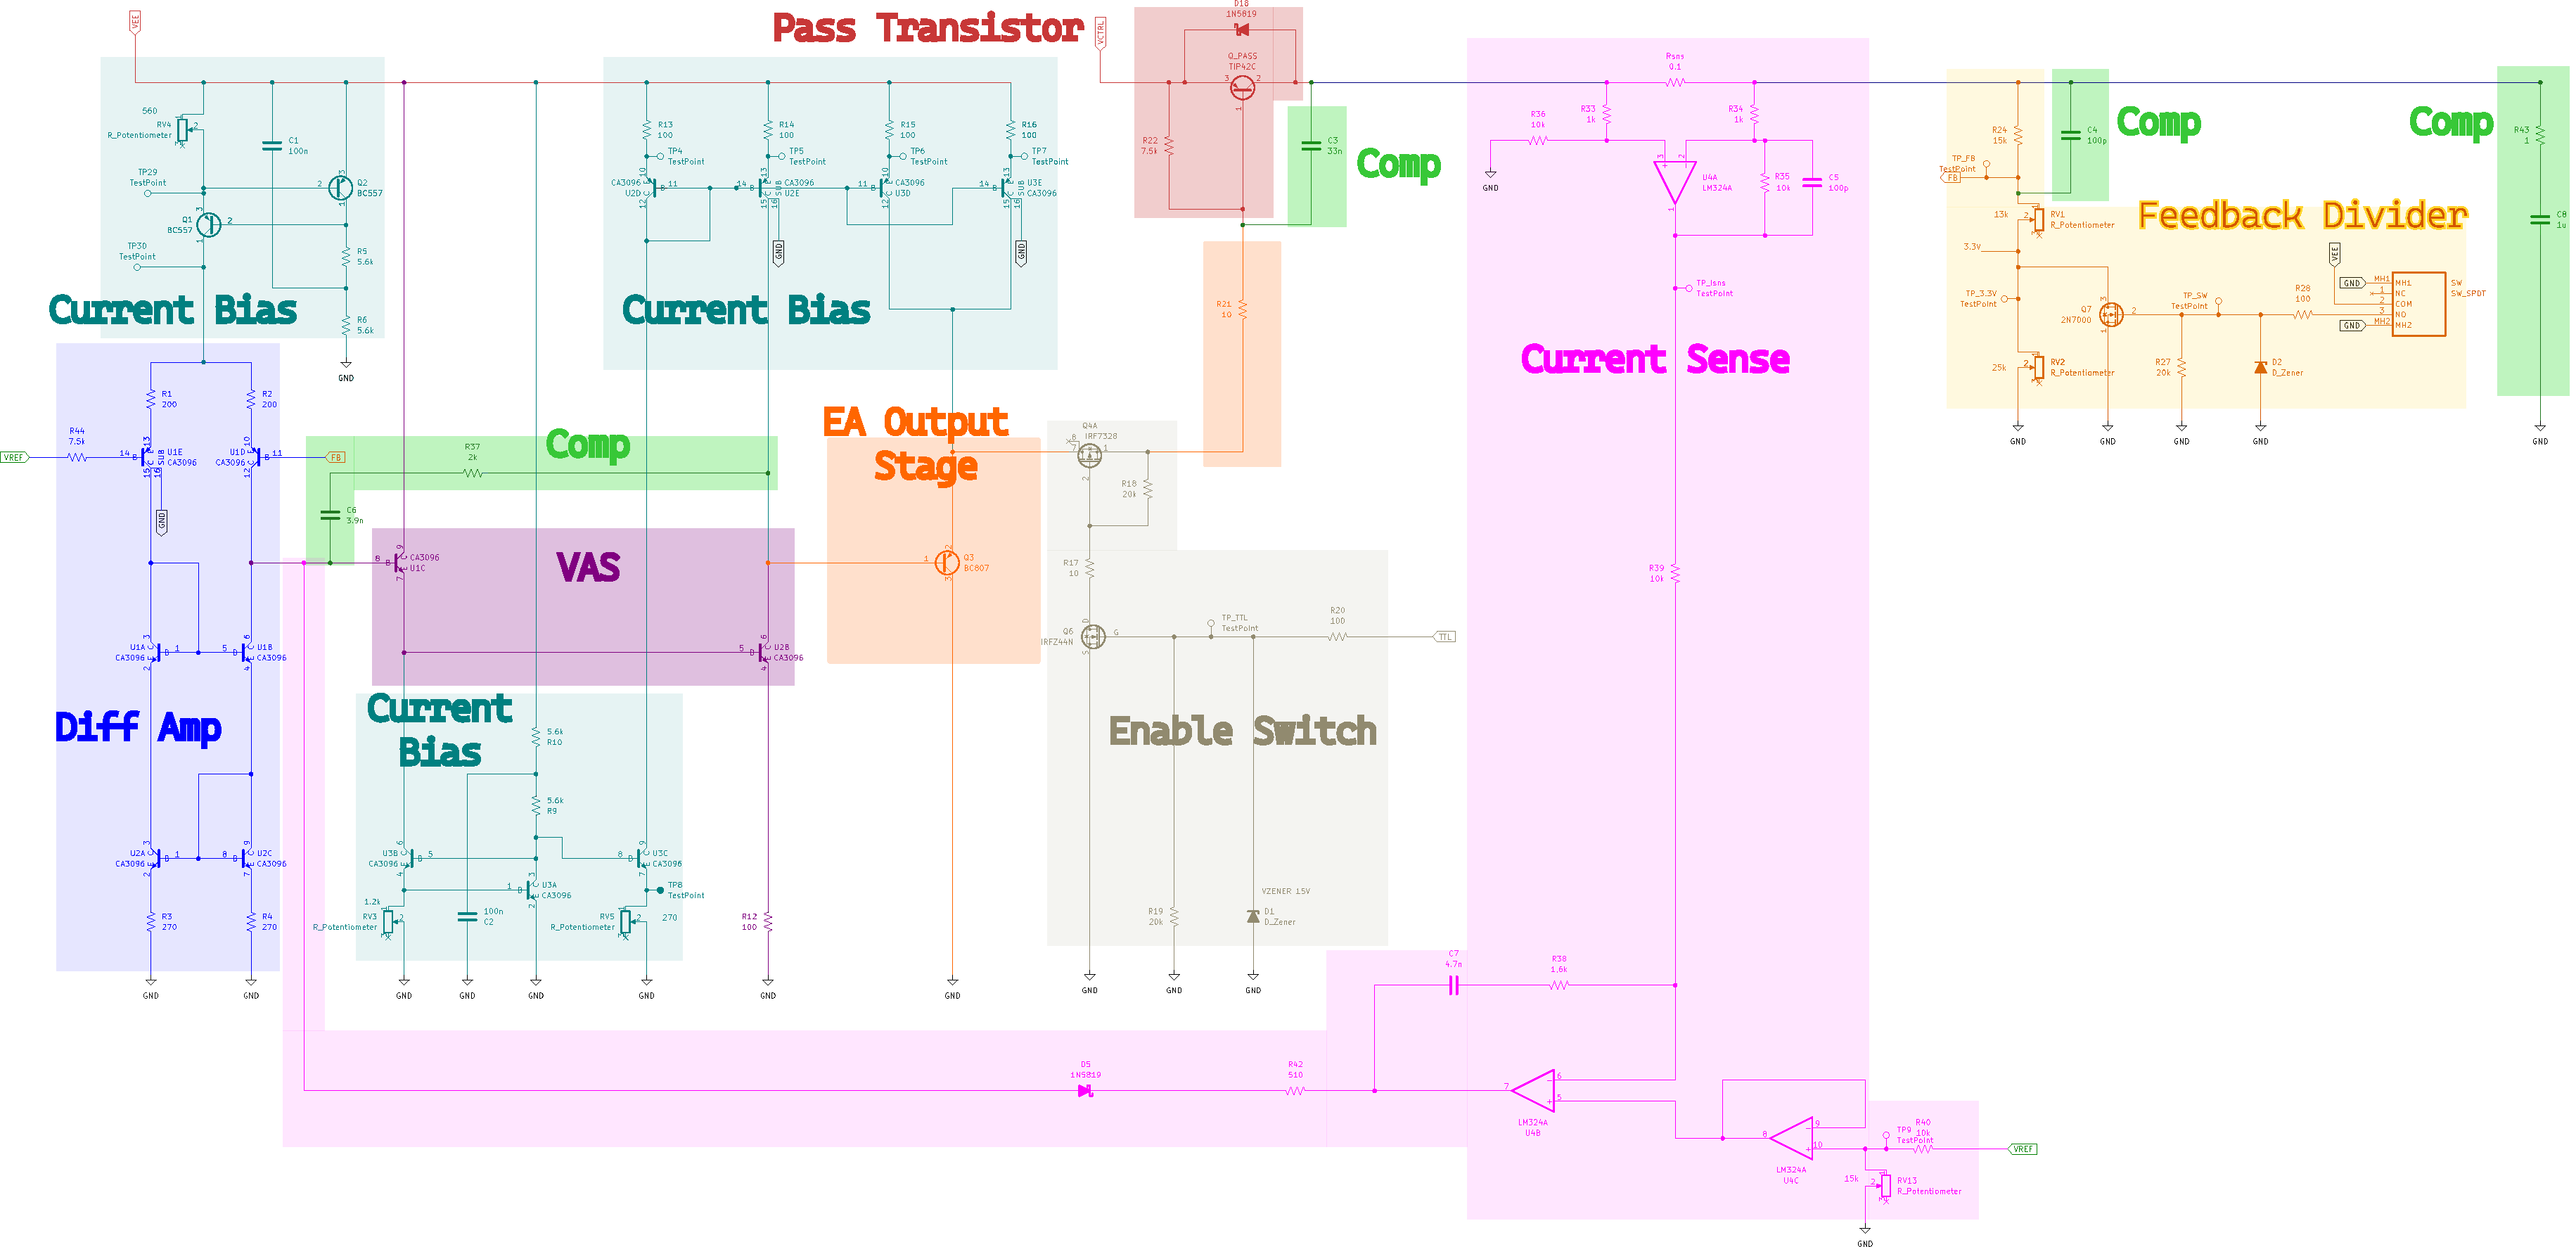
\includegraphics[width=0.95\textwidth]{EAIMG.pdf}
    \caption{Annotated schematic of the regulation stage,
    showing the error amplifier, bias circuits, pass
    transistor, feedback network, compensation components,
    enable switch, and current-limit circuit.}
    \label{fig:error_amplifier_detail}
\end{figure*}

The differential input pair is formed by the two PNP
transistors U1D and U1E within the same CA3096E transistor
array. These devices compare \(V_{\mathrm{fb}}\) and
\(V_{\mathrm{ref}}\), converting their difference into
collector-current variations. The CA3096 integrates its
transistors on a common substrate
\cite{harris_ca3096_1996}. Using both input devices within
the same array was intended to promote thermal tracking
and reduce their exposure to different local temperatures.

The input pair is loaded by a four-transistor Wilson
current mirror formed by U1A, U1B, U2A, and U2C.
This active load combines the collector-current variations
of the input pair into a single-ended signal that drives
the VAS. The Wilson configuration reduces the
current-transfer error associated with finite transistor
current gain. Its four-transistor form also equalizes
the collector--emitter voltages of the two devices
forming the internal mirror, reducing the influence of
the Early effect on current matching
\cite{self_audio_power_2009}.

The VAS consists of the emitter follower U1C followed
by the common-emitter transistor U2B. This arrangement
increases the effective current gain of the VAS.
Because U1C is enclosed within the local feedback loop
through the Miller compensation capacitor C6, the
additional gain increases local negative feedback,
improving VAS linearity and reducing its output
impedance \cite{self_audio_power_2009}. The surrounding
current-source and current-mirror circuits establish
the bias conditions of the amplifier stages.

The EA output stage uses the PNP transistor Q3 as an
emitter follower with an active current-source load,
biased for Class-A operation. In this operating class,
the output devices remain conducting throughout the
signal excursion, avoiding the turn-on and turn-off
transitions associated with cutoff
\cite{self_audio_power_2009}. In the present circuit,
the emitter of Q3 is connected to the base of
\(Q_{\mathrm{pass}}\) through the enable switch Q4A
and the series resistor R21. When the regulator is
enabled, Q3 sinks current from this path to control
the conduction of the pass transistor. Resistor R22,
connected between the base and emitter of
\(Q_{\mathrm{pass}}\), provides a pull-up path to
turn it off when the drive is disconnected.

With Q4A conducting, and neglecting the voltage drops
across Q4A and R21, the base voltage of Q3 is approximately
\[
V_{B,Q_3}
\approx
V_{\mathrm{in}}
-
V_{EB,Q_{\mathrm{pass}}}
-
V_{EB,Q_3}.
\]
This relation describes the voltage level at the VAS
output during normal conduction.

Capacitor C6 provides a feedback path between the VAS
output and the differential-stage output. Together with
the other compensation components identified in
Fig.~\ref{fig:error_amplifier_detail}, it shapes the
frequency response of the regulation loop. These
components were included to obtain stable operation
and a suitable transient response; the simulated
load-step results are reported in the electrical
characteristics section.

The output uses a 1\,$\mu$F tantalum capacitor with an external
1\,$\Omega$ series resistor. This resistor deliberately adds series
resistance independently of the capacitor's intrinsic ESR. Series
resistance can introduce a zero that assists loop compensation;
Texas Instruments illustrates this technique by adding a discrete
1\,$\Omega$ resistor to an output capacitor
\cite{ti_esr_stability_2020}. The present design is evaluated using
its own simulated loop response; the nominal model includes the
external resistor but neglects the capacitor's additional ESR.

The figure also includes the current-limit circuit,
which senses the voltage across \(R_{\mathrm{sns}}\)
and acts on the differential-stage output through
\(D_5\). Its operation and threshold setting are
described in the protection-circuit subsection.

\subsection{Reference Stage}

The reference stage uses two independently biased TL431
programmable shunt references, U5 and U8, each configured
to provide approximately 2.5\,V
\cite{ti_tl431_2024}. Each device is supplied by a BJT
current source whose current-setting resistor has
approximately one base--emitter voltage across it.
Neglecting base currents, the resulting bias current
is approximately
\[
I_{\mathrm{bias}}
\approx
\frac{V_{BE}}{R_{\mathrm{set}}},
\]
where \(R_{\mathrm{set}}\) is the effective resistance
of the corresponding adjustment potentiometer.

Compared with a simple series resistor, this arrangement
reduces the dependence of the supplied current on
\(V_{\mathrm{in}}\), provided that the current source
has sufficient voltage headroom. The bias current must
supply the connected reference loads while maintaining
the cathode current required by the TL431 for regulation
\cite{ti_tl431_2024}.

U5 generates \(V_{\mathrm{ref}}\) for the error amplifier.
The enable-controlled MOSFET network can pull this
reference toward ground to disable the regulation
command. This action complements the disconnection
of the pass-transistor drive described in the
enable-control subsection.

U8 supplies the reference used by the UVLO/OVLO protection
circuits, labeled ``UVLO/OVLO reference'' in the simulation
plots. Its bias is independent
of the main-reference disable path, allowing the
protection circuitry to retain its reference when
\(V_{\mathrm{ref}}\) is disabled, provided that the
input supply is sufficient to bias the auxiliary
reference.

\subsection{Output-Voltage Selection}

The regulator selects between \(5\,\mathrm{V}\) and
\(3.3\,\mathrm{V}\) by reconfiguring the feedback divider,
which consists of R24 and the adjustment potentiometers
RV1 and RV2. The 2N7000 NMOS transistor Q7 is connected
across RV2 and acts as the selection switch.

When Q7 is turned on, it bypasses RV2, leaving RV1
as the lower divider resistance and selecting the
5\,V output. When Q7 is turned off, RV2 remains in
series with RV1, increasing the lower divider
resistance and selecting the 3.3\,V output.

The regulation loop adjusts the conduction of
\(Q_{\mathrm{pass}}\) until \(V_{\mathrm{fb}}\)
approaches \(V_{\mathrm{ref}}\). Neglecting the
feedback-input current, the on-state resistance
of Q7, and its off-state leakage, the two output
settings are approximately
\[
V_{\mathrm{out,5V}}
\approx
V_{\mathrm{ref}}
\left(
1+\frac{R_{24}}{R_{\mathrm{V1}}}
\right),
\]
\[
V_{\mathrm{out,3.3V}}
\approx
V_{\mathrm{ref}}
\left(
1+\frac{R_{24}}{R_{\mathrm{V1}}+R_{\mathrm{V2}}}
\right),
\]
where \(R_{\mathrm{V1}}\) and \(R_{\mathrm{V2}}\)
denote the effective resistances set by RV1 and RV2.

This arrangement allows the 5\,V setting to be
adjusted first using RV1 with Q7 on. The 3.3\,V
setting can then be adjusted using RV2 with Q7 off,
without changing the previously established
5\,V setting under the stated approximations.

\subsection{Enable Control}

The enable circuit implements a three-input AND function
using discrete transistors. The series-connected BC547
transistors Q25, Q26, and Q27, together with a collector
pull-up resistor, form a NAND stage. Their inputs represent
the undervoltage, overvoltage, and startup-delay conditions,
with a high level indicating that the corresponding
condition permits operation. Transistor Q23 inverts the
NAND output, producing a high enable signal only when
all three conditions are satisfied.

The enable signal drives the IRFZ44N N-channel MOSFET
Q6, which pulls down the gate of the P-channel switch
Q4A within the IRF7328. When Q4A conducts, it connects
the error-amplifier output stage to the base-drive
path of \(Q_{\mathrm{pass}}\) through R21, allowing
the feedback loop to regulate the output voltage.

If any enable condition is lost, Q6 turns off and
the gate-bias network returns Q4A to its off state.
This disconnects the error-amplifier drive, while
R22 pulls the base of \(Q_{\mathrm{pass}}\) toward
its emitter to turn the pass transistor off.
The enable signal also controls the main-reference
disable circuit described in the preceding subsection.

This arrangement requires both input-voltage protection
circuits to permit operation and the startup delay
to have elapsed before enabling the regulator.

\subsection{Protection Circuits}

The protection circuitry monitors the input voltage
and the output current. Input-voltage faults disable
the regulator through the enable circuit, while the
current-limit circuit acts on the error amplifier
to restrict the current delivered by the pass transistor.

The UVLO circuit uses one section of an LM339 comparator.
Its inverting input is connected to the auxiliary
reference, while its non-inverting input senses
\(V_{\mathrm{in}}\) through a resistive divider.
The divider includes potentiometers that allow the
switching thresholds to be calibrated, compensating
for component tolerances.

An NMOS switching network changes the effective
resistance of the UVLO divider according to the
comparator output state. This introduces hysteresis,
with a higher input voltage required to enable
operation than to maintain it. The separation between
the turn-on and turn-off thresholds reduces repeated
switching caused by small input-voltage fluctuations
near the undervoltage limit \cite{sachdev_hysteresis_2021}.

The OVLO circuit uses one section of an LM324
operational amplifier as a comparator, with its
non-inverting input connected to the auxiliary
reference and its inverting input connected to
the input-sensing divider. Its output removes
the enable permission when \(V_{\mathrm{in}}\)
exceeds the upper threshold. An NMOS-switched
divider branch introduces hysteresis, requiring
the input voltage to fall below a lower threshold
before operation is permitted again. Potentiometers
allow these thresholds to be adjusted.

In both protections, switching a divider resistor provides
state-dependent feedback and distinct rising and falling
thresholds, following the switched-resistor hysteresis principle
described in \cite{sachdev_hysteresis_2021}.

The current-sense circuit uses a
\(0.1\,\Omega\) resistor in the output-current path.
The voltage across this resistor is
\[
V_{\mathrm{sns}}
=
I_{\mathrm{sns}}R_{\mathrm{sns}},
\]
where \(I_{\mathrm{sns}}\) is the current through
the sense resistor, approximately equal to the
load current when the current drawn by the
output-connected sensing networks is neglected.

The LM324 differential stage U4A amplifies this
voltage with a nominal DC gain of 10, giving
\[
V_{\mathrm{cs}}
\approx
10 I_{\mathrm{out}}R_{\mathrm{sns}}.
\]
Consequently, an output current of
\(1.5\,\mathrm{A}\) produces approximately
\(1.5\,\mathrm{V}\) at the current-sense output.

The current-limit threshold \(V_{\mathrm{lim}}\)
is derived from the main reference \(V_{\mathrm{ref}}\)
through R40 and potentiometer RV13, and buffered
by the LM324 voltage follower U4C. RV13 allows
the current limit to be calibrated. Neglecting
sensing and amplifier errors, the limit is
approximately
\[
I_{\mathrm{lim}}
\approx
\frac{V_{\mathrm{lim}}}{10R_{\mathrm{sns}}}.
\]

The LM324 section U4B compares the amplified
current-sense voltage with \(V_{\mathrm{lim}}\)
and provides the control signal for current limiting.
The R38--C7 feedback network shapes its dynamic
response. When \(V_{\mathrm{cs}}\) exceeds the
threshold, the output of U4B moves downward,
forward biasing \(D_5\) and drawing current from
the single-ended output of the error-amplifier
input stage through R42.

During normal voltage regulation, \(D_5\) is
nonconducting, isolating the current-limit control
path from the error amplifier. When the limit is
reached, this path modifies the pass-transistor
drive to restrict the output current, allowing
the output voltage to decrease as required.

\subsection{Input Polarity Protection}

A P-channel 4905 MOSFET at the input provides protection
against reverse supply polarity. This stage precedes
the startup circuit and the remaining regulator circuitry.

\subsection{Startup and Enable Sequencing}

The startup circuit controls the rate of rise of the
internal supply voltage through active feedback. This node,
at the output of the startup circuit, is labeled
``Startup-circuit output'' in the simulation plots.
A capacitor--resistor network senses changes in this
voltage and drives a BJT control stage, which adjusts
the gate voltage of the series P-channel MOSFET to
oppose excessively rapid increases
\cite{lathrop_soft_start}.

Slope control becomes effective only after the BJT
stage develops sufficient bias. Consequently, startup
includes an initial rapid voltage rise followed by
a controlled ramp. In the simulated implementation,
the transition to the controlled ramp occurs at
approximately 2.2\,V. The initial charging-current
peak depends on the supply impedance, capacitor ESR,
and other parasitic elements.

A separate time-delay circuit postpones regulator
enablement to allow the references and input-voltage
protection circuits to establish their operating
conditions. Its output forms one of the three inputs
to the enable logic, together with the UVLO and OVLO
permission signals. The regulator is therefore enabled
only after the delay has elapsed and both protection
circuits permit operation.

Separating the supply ramp from the enable delay
allows the internal circuitry to become biased before
the output-regulation loop is enabled.

\subsection{Shutdown and Capacitor Discharge}

Two P-channel JFET discharge paths are provided:
one at the internal supply node following the startup
circuit, and another at \(V_{\mathrm{out}}\).
These paths discharge the stored capacitor energy
when the corresponding node is no longer required
to remain powered.

The JFETs were selected for their normally-on behavior:
they conduct at zero gate--source voltage, allowing
the discharge paths to operate without an auxiliary
supply to turn them on after input power is removed.
During normal operation, a voltage doubler supplies
the gate-control circuitry with sufficient voltage
to bias the JFETs into cutoff.

The two discharge paths use different control conditions.
The internal-supply discharge path is governed by the
startup timing sequence and remains inactive while
sufficient input voltage is available. It discharges
the \(10\,\mu\mathrm{F}\) capacitor following removal
of the input supply.

The output discharge path is controlled by a comparator
using the three-input AND enable signal. It remains
inactive while the regulator is enabled and is activated
when enable permission is removed, including shutdown
due to UVLO or OVLO. This provides a discharge path
for the output capacitor in addition to disconnecting
the pass-transistor drive.

% ======================================================================
% ELECTRICAL CHARACTERISTICS
% ======================================================================
\section{Electrical Characteristics}

The regulator was evaluated through LTspice simulations
covering startup and shutdown, steady-state regulation,
load transients, and protection operation. The following
results characterize the simulated design and provide
a basis for comparison with hardware measurements.

\subsection{Simulation Conditions}

Unless otherwise stated, simulations were performed
at \(27\,^{\circ}\mathrm{C}\) using the component values
and device models in the corresponding test schematic.
The input voltage, load, and output-voltage setting
are specified for each test. Reported values apply
to these simulated conditions and do not represent
guaranteed limits over component tolerances or temperature.
The simulations include the nonidealities represented by the
device models and explicitly specified circuit elements, but do
not comprehensively model PCB and wiring parasitics, source and
load impedances, or self-heating. Component tolerances and thermal
variation were not swept. The curves therefore describe the
modeled circuit under nominal conditions and require comparison
with measurements on the assembled board.

\subsection{Startup and Shutdown Behavior}

\begin{figure*}[t]
\centering
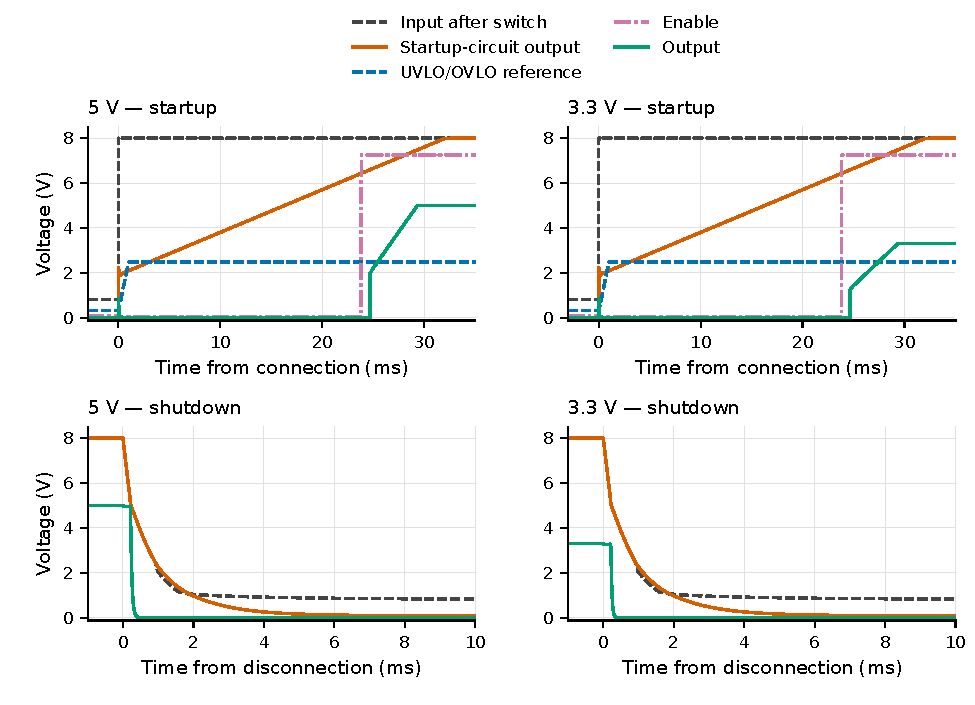
\includegraphics[width=0.95\textwidth]{SIM-01_calibrated_startup.pdf}
\caption{Calibrated startup and shutdown (SIM-01): 8\,V source,
27\,\textdegree C, 50\,$\Omega$ load in 5\,V mode and
33\,$\Omega$ in 3.3\,V mode. Time origins are input connection
and disconnection, respectively. Input after switch denotes the
node downstream of the series test switch.}
\label{fig:startup_shutdown}
\end{figure*}

Figure~\ref{fig:startup_shutdown} shows the recalibrated SIM-01
in both output modes at \(27\,^{\circ}\mathrm{C}\), with an
\(8\,\mathrm{V}\) source and resistive loads of
\(50\,\Omega\) and \(33\,\Omega\), respectively
(approximately \(0.1\,\mathrm{A}\)). The feedback adjustment
matches SIM-02; the lighter load is chosen to examine sequencing.
The input switch connects at \(5\,\mathrm{ms}\), opens at
\(55\,\mathrm{ms}\), and reconnects at \(85\,\mathrm{ms}\).
The complete record extends to \(140\,\mathrm{ms}\).
Opening the switch does not force the downstream input node to ground.

The enable signal crosses \(3.5\,\mathrm{V}\) after
23.82 and 23.82\,ms from connection in the 5\,V and
3.3\,V modes. These are timing conventions rather than specified
logic thresholds. After enable, the output first reaches 98\% of
nominal at 29.19 and 29.19\,ms from connection;
its mean over 45--55\,ms is 5.0000 and 3.3000\,V.
Figure~\ref{fig:initial_transient} resolves the initial
startup-circuit step and the pre-enable output pulse. The latter
reaches approximately 0.86 and 0.84\,V in the two modes.
The initial step is consistent with the bias requirement of the
BJT slope-control stage described earlier.

After disconnection, the output first falls below
\(50\,\mathrm{mV}\) in 0.39 and 0.33\,ms;
the startup-circuit output reaches the same level in
12.48 and 12.48\,ms. The figure shows the first
\(10\,\mathrm{ms}\) of shutdown; discharge times are extracted
from the full record. Both modes recover regulation after reconnection.

The load is represented as a constant behavioral resistance,
electrically equivalent to the stated resistor. The complete 140\,ms sequence was rerun with the IRF4905
input-protection model and a 2\,$\mu$s maximum timestep.
Source impedance, switch behavior and capacitor ESR
must be characterized for a hardware comparison; in particular,
C11 has no explicitly specified ESR in this model. These results
characterize nominal sequencing, not hardware inrush-current limits.



\begin{figure}[H]
\centering
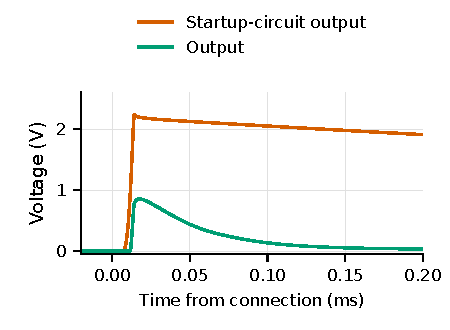
\includegraphics[width=\columnwidth]{SIM-01_calibrated_initial.pdf}
\caption{Initial connection transient of recalibrated SIM-01
in 5\,V mode: startup-circuit output and regulator output,
with an 8\,V source, 50\,$\Omega$ load and 27\,\textdegree C.}
\label{fig:initial_transient}
\end{figure}

\begin{figure*}[t]
    \centering
    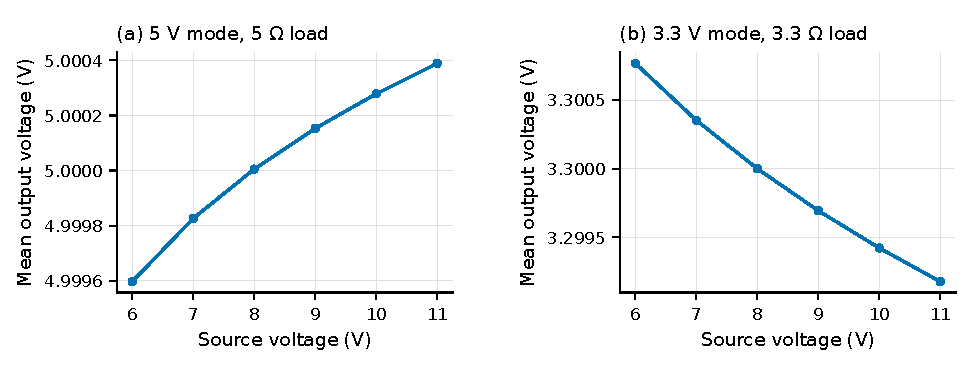
\includegraphics[width=0.95\textwidth]{SIM-02_calibrated_line.pdf}
    \caption{Full-circuit line regulation after calibration (SIM-02),
    at \(27\,^{\circ}\mathrm{C}\). Markers show final-window
    transient averages, with lines connecting sampled points.
    Both panels use expanded output-voltage scales; loads are resistive.}
    \label{fig:line_regulation}
\end{figure*}

\subsection{DC Characteristics}

Figure~\ref{fig:line_regulation} shows the calibrated complete
circuit in both output modes (SIM-02). The two adjustable divider
resistances are \(14.8465\,\mathrm{k\Omega}\) and
\(28.7598\,\mathrm{k\Omega}\), unchanged between modes and
throughout the test. At an \(8\,\mathrm{V}\) source
and \(27\,^{\circ}\mathrm{C}\) the mean outputs are
\(5.00000\,\mathrm{V}\) and \(3.30000\,\mathrm{V}\), with
\(5\,\Omega\) and \(3.3\,\Omega\) loads, respectively
(approximately \(1\,\mathrm{A}\)).

Each transient run starts at \(8\,\mathrm{V}\), then visits
\(6\)--\(11\,\mathrm{V}\) in \(1\,\mathrm{V}\) increments.
Input transitions take \(0.1\,\mathrm{ms}\), with
\(40\,\mathrm{ms}\) between changes. The plotted values are
averages over the final \(10\,\mathrm{ms}\) of each interval.
The horizontal axis denotes the source before the series input
switch. All protection and enable circuits remain active.
Adjacent-window output means differ by less than
\(0.001\,\mathrm{mV}\), and the repeated \(8\,\mathrm{V}\)
point agrees with its initial value within \(1\,\mu\mathrm{V}\).

The line-regulation magnitude is calculated from the endpoints:
\[
S_{\mathrm{line}} =
\left|\frac{\overline{V}_{\mathrm{out}}(11\,\mathrm{V})-
\overline{V}_{\mathrm{out}}(6\,\mathrm{V})}{11\,\mathrm{V}-6\,\mathrm{V}}\right|.
\]
The resulting values are \(0.159\,\mathrm{mV/V}\) in the
\(5\,\mathrm{V}\) mode and \(0.319\,\mathrm{mV/V}\) in the
\(3.3\,\mathrm{V}\) mode. These nominal-model results
characterize settled operation following input changes; they do
not establish hardware accuracy or startup performance at every
input voltage.




\begin{figure*}[t]
    \centering
    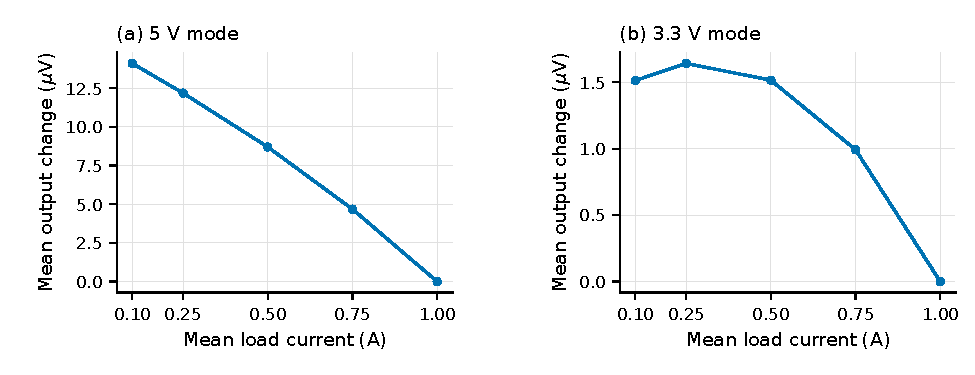
\includegraphics[width=0.95\textwidth]{SIM-03_calibrated_load.pdf}
    \caption{Settled load regulation of the calibrated complete
    circuit (SIM-03), with an \(8\,\mathrm{V}\) source and
    \(27\,^{\circ}\mathrm{C}\). Markers are final-window averages
    of actual load current and output-voltage change relative to the
    final \(1\,\mathrm{A}\) point; lines connect sampled points.
    The two panels use different vertical scales.}
    \label{fig:load_regulation}
\end{figure*}

Load regulation was evaluated with the same calibration at an
\(8\,\mathrm{V}\) source (SIM-03). Five resistive loads span
approximately \(0.1\)--\(1\,\mathrm{A}\), with nominal intermediate
currents of \(0.25\), \(0.5\), and \(0.75\,\mathrm{A}\)
(Fig.~\ref{fig:load_regulation}). Each point is held for
\(40\,\mathrm{ms}\), and voltage and current are averaged over
the final \(10\,\mathrm{ms}\). The actual simulated load current
is used in the calculation:
\[
S_{\mathrm{load}}=
\left|\frac{\Delta\overline{V}_{\mathrm{out}}}
{\Delta\overline{I}_{\mathrm{load}}}\right|.
\]
The endpoint magnitudes are \(0.017\,\mathrm{mV/A}\) and
\(<0.001\,\mathrm{mV/A}\) for the \(5\,\mathrm{V}\) and
\(3.3\,\mathrm{V}\) modes, respectively. The regulator remains
enabled at all points; adjacent-window voltage means differ by
less than \(0.001\,\mathrm{mV}\). Returning to the initial
\(1\,\mathrm{A}\) load reproduces its mean output within
\(1\,\mu\mathrm{V}\). These results describe settled regulation;
load-step undershoot and overshoot are separate characteristics.
These nominal-model averages do not establish comparable hardware
accuracy or thermal performance.


In SIM-05, the complete enabled regulator draws a mean input current
of \(56.9\,\mathrm{mA}\) in the 5\,V mode and
\(56.0\,\mathrm{mA}\) in the 3.3\,V mode, from an 8\,V source.
A \(1\,\mathrm{M}\Omega\) external load approximates no-load
operation, drawing about \(5\,\mu\mathrm{A}\) and
\(3.3\,\mu\mathrm{A}\), respectively. The reported current
includes this load and all auxiliary circuits; it is not the
error-amplifier bias current alone. Time-weighted averages use
100--120\,ms after startup; four consecutive 10\,ms windows
from 80--120\,ms agree within \(0.02\,\mathrm{mA}\).
Both outputs remain regulated. Shutdown consumption is not
characterized by this enabled-state test.

\begin{table*}[t]
\centering
\footnotesize
\setlength{\tabcolsep}{4pt}
\caption{DC electrical characteristics (LTspice, 27\,\textdegree C)}
\label{tab:dc_characteristics}
\begin{tabularx}{\textwidth}{@{}L{1.4cm}L{3.8cm}Xccc@{}}
\toprule
\textbf{Mode} & \textbf{Parameter} & \textbf{Conditions} & \textbf{Min} & \textbf{Typ} & \textbf{Max} \\
\midrule

5\,V & Output voltage window &
$V_{IN}=6$--$11$\,V, $R_{LOAD}=5\,\Omega$, calibrated SIM-02 &
4.99959\,V & -- & 5.00039\,V \\

5\,V & Deviation from nominal &
$V_{IN}=6$--$11$\,V, maximum sampled mean deviation from 5.000\,V, calibrated SIM-02 &
-- & -- & $0.0081\%$ \\

5\,V & Line regulation &
$V_{IN}=6$--$11$\,V, $R_{LOAD}=5\,\Omega$, endpoint magnitude, calibrated SIM-02 &
-- & 0.159\,mV/V & -- \\

5\,V & Load regulation &
$V_{IN}=8$\,V, $I_{LOAD}\approx0.1$--$1$\,A, settled means, SIM-03 &
-- & 0.017\,mV/A & -- \\

5\,V & Output change with load &
$V_{IN}=8$\,V, $I_{LOAD}\approx0.1$--$1$\,A, settled means, SIM-03, high minus low load &
-- & -0.015\,mV & -- \\



5\,V & Near-no-load input current &
8\,V source, 1\,M$\Omega$ load, enabled complete circuit, SIM-05 &
-- & 56.9\,mA & -- \\

\midrule

3.3\,V & Output voltage window &
$V_{IN}=6$--$11$\,V, $R_{LOAD}=3.3\,\Omega$, calibrated SIM-02 &
3.29918\,V & -- & 3.30077\,V \\

3.3\,V & Deviation from nominal &
$V_{IN}=6$--$11$\,V, maximum sampled mean deviation from 3.300\,V, calibrated SIM-02 &
-- & -- & $0.0249\%$ \\

3.3\,V & Line regulation &
$V_{IN}=6$--$11$\,V, $R_{LOAD}=3.3\,\Omega$, endpoint magnitude, calibrated SIM-02 &
-- & 0.319\,mV/V & -- \\

3.3\,V & Load regulation &
$V_{IN}=8$\,V, $I_{LOAD}\approx0.1$--$1$\,A, settled means, SIM-03 &
-- & $<0.001$\,mV/A & -- \\

3.3\,V & Output change with load &
$V_{IN}=8$\,V, $I_{LOAD}\approx0.1$--$1$\,A, settled means, SIM-03, high minus low load &
-- & $|\Delta V|<0.001$\,mV & -- \\



3.3\,V & Near-no-load input current &
8\,V source, 1\,M$\Omega$ load, enabled complete circuit, SIM-05 &
-- & 56.0\,mA & -- \\

\bottomrule
\end{tabularx}
\vspace{1mm}

\parbox{0.95\textwidth}{\footnotesize\emph{Note: SIM-02 and SIM-03 use the calibrated complete circuit; sampled extrema are not tolerance limits. Load regulation uses settled transient averages; the signed output change is the high-load mean minus the low-load mean. SIM-05 reports total source-current averages with a 1 M$\Omega$ external load and all auxiliary blocks active. The nominal-threshold SIM-04 test disables before dropout; an adjusted-threshold exploration is discussed separately. Hardware results may differ due to component tolerances, parasitic resistances, temperature drift, and measurement uncertainty.}}
\end{table*}


% ----------------------------------------------------------------------
% Transient characteristics
% ----------------------------------------------------------------------


\begin{figure*}[t]
    \centering
    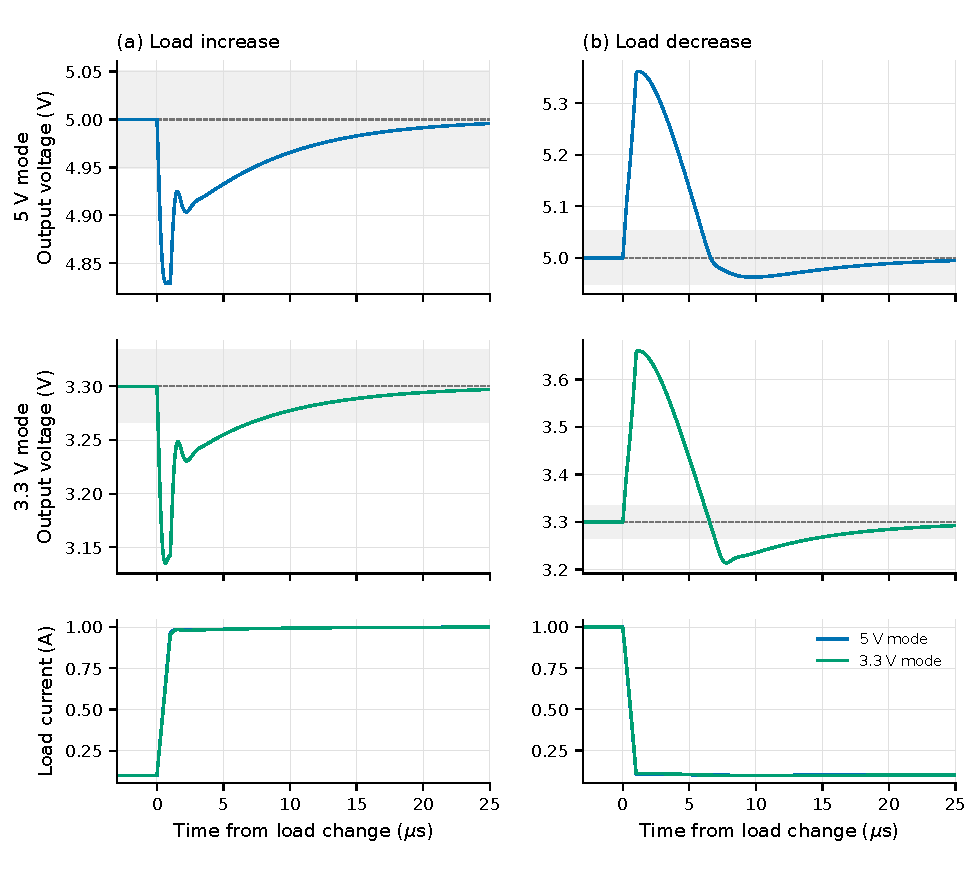
\includegraphics[width=0.95\textwidth]{SIM-06_calibrated_transient.pdf}
    \caption{Calibrated full-circuit response to a resistive load increase
    and decrease (SIM-06), with an \(8\,\mathrm{V}\) source and
    \(27\,^{\circ}\mathrm{C}\). Load conductance changes in
    \(1\,\mu\mathrm{s}\); the bottom row shows actual load current.
    Time is relative to the start of each transition. Dashed lines
    indicate final mean outputs; shading denotes the \(\pm1\%\) bands.}
    \label{fig:load_transient}
\end{figure*}

\subsection{Transient Characteristics}

Figure~\ref{fig:load_transient} shows the calibrated complete
circuit under load changes of approximately \(0.1\rightarrow1\,\mathrm{A}\)
and \(1\rightarrow0.1\,\mathrm{A}\) (SIM-06). The load resistance
changes between \(50\) and \(5\,\Omega\) in the \(5\,\mathrm{V}\)
mode, and between \(33\) and \(3.3\,\Omega\) in the
\(3.3\,\mathrm{V}\) mode. Conductance ramps in
\(1\,\mu\mathrm{s}\); actual current also responds to the output
voltage. Transitions occur at \(80\) and \(120\,\mathrm{ms}\),
after startup and with the source held at \(8\,\mathrm{V}\).

Undershoot and overshoot are measured relative to the final
\(10\,\mathrm{ms}\) mean for each load. Settling time is measured
from the start of the conductance ramp to the last entry into
a \(\pm1\%\) band about that mean, with the output remaining
inside the band for the rest of the observation interval.
Samples near each transition are separated by at most
\(20\,\mathrm{ns}\). The regulator remains enabled throughout
both transitions. Table~\ref{tab:transient_characteristics}
summarizes these nominal-model results; they do not establish
hardware response or frequency-domain stability margins.
In the \(3.3\,\mathrm{V}\) mode, load removal produces an
overshoot followed by an undershoot that also leaves the
\(\pm1\%\) band, extending the measured recovery time.

\begin{table*}[t]
\centering
\footnotesize
\setlength{\tabcolsep}{4pt}
\caption{Calibrated full-circuit transient characteristics
(SIM-06, \(8\,\mathrm{V}\) source, \(27\,^{\circ}\mathrm{C}\),
\(1\,\mu\mathrm{s}\) conductance transitions)}
\label{tab:transient_characteristics}
\begin{tabularx}{\textwidth}{@{}L{1.4cm}L{4.0cm}Xcc@{}}
\toprule
\textbf{Mode} & \textbf{Parameter} & \textbf{Conditions} & \textbf{Typ} & \textbf{Unit} \\
\midrule
5\,V & Load range &
Settled currents before and after the increase &
0.100--1.000 & A \\

5\,V & Step-up undershoot &
Final mean minus minimum output &
172.2 / 3.44 & mV / \% \\

5\,V & Step-down overshoot &
Maximum output minus final mean &
362.7 / 7.25 & mV / \% \\

5\,V & Settling time, step-up &
Last entry into final \(\pm1\%\) band &
7.42 & \(\mu\)s \\

5\,V & Settling time, step-down &
Last entry into final \(\pm1\%\) band &
6.02 & \(\mu\)s \\

\midrule
3.3\,V & Load range &
Settled currents before and after the increase &
0.100--1.000 & A \\

3.3\,V & Step-up undershoot &
Final mean minus minimum output &
164.8 / 4.99 & mV / \% \\

3.3\,V & Step-down overshoot &
Maximum output minus final mean &
361.1 / 10.94 & mV / \% \\

3.3\,V & Settling time, step-up &
Last entry into final \(\pm1\%\) band &
7.40 & \(\mu\)s \\

3.3\,V & Settling time, step-down &
Last entry into final \(\pm1\%\) band &
14.80 & \(\mu\)s \\

\bottomrule
\end{tabularx}
\end{table*}

\subsection{Regulation-Loop Stability}

SIM-09 evaluates the nominal small-signal regulation loop at
approximately \(1\,\mathrm{A}\) in each output mode. The bench
retains the discrete amplifier, pass transistor, feedback network,
compensation, output capacitor, and current-limit path. Supplies,
reference and enable are held at steady bias values corresponding
to the complete circuit with an \(8\,\mathrm{V}\) source;
the switching doubler and sequencing dynamics are excluded.
The bench is allowed to settle before linearization about its steady-state operating point. DC bias determines the device small-signal parameters; the frequency sweep describes incremental variations around that bias. Holding the auxiliary sources fixed additionally neglects their small-signal impedance and coupling, rather than merely removing a DC offset.

Voltage and current injections between the feedback divider and
the amplifier input give the return ratio using Tian's method
\cite{tian_stability_2001}. With the critical point at \(-1\),
phase margin is \(180^{\circ}+\angle T\) at unity magnitude;
gain margin is \(-20\log_{10}|T|\) at \(-180^{\circ}\).
Figure~\ref{fig:regulation_loop_gain} and
Table~\ref{tab:loop_stability} show the resulting positive margins.
Increasing the frequency sampling density tenfold and reversing the
probe orientation leave the reported rounded margins unchanged.

As a limited cross-check, a \(500\,\mu\mathrm{V}\) sinusoid
was injected into the complete switching circuit at each calculated
crossover frequency. A fit over the final 80 cycles gives a
voltage-return response that agrees with the
same voltage-return quantity from the AC bench within
0.04\,dB and 1.3\,degrees. This single-frequency
check does not validate the entire frequency sweep or the stability
of every internal loop.

A separate load-sensitivity check keeps the auxiliary biases fixed
and recalculates the operating point for each load. At approximately
0.1\,A, phase margins are 57.3\textdegree{} and 53.8\textdegree{}
for the 5\,V and 3.3\,V modes. With a 1\,M$\Omega$ external load,
they decrease to 41.5\textdegree{} and 31.7\textdegree{}, while
crossover frequencies fall to 19.5 and 17.1\,kHz. These checks retain
the 1\,$\mu$F output capacitor and external 1\,$\Omega$ series resistor. They show
load dependence but do not establish margins for every intermediate
load, temperature, component tolerance or auxiliary-supply condition.

Output-capacitor sensitivity was also examined, motivated by the
influence of capacitance and ESR on regulator loop dynamics
\cite{ti_esr_stability_2020}. With a 1\,M$\Omega$ load and the output
auxiliary branch retained, varying capacitance from 0.8 to
1.2\,$\mu$F at 1\,$\Omega$ modeled series resistance gives phase margins of
43.9--39.7\textdegree{} (5\,V) and 33.3--30.6\textdegree{}
(3.3\,V). A hypothetical reduction of total modeled series
resistance to 0.1\,$\Omega$ at 1\,$\mu$F lowers
the 3.3\,V margin to 26.4\textdegree{}. Small added-load transients
in this fixed-bias bench show decaying ringing, more pronounced
with the lower series resistance. The 0.1\,$\Omega$ case does
not represent the board with its external 1\,$\Omega$ resistor.
The capacitor's intrinsic ESR adds to that resistance; these tests
do not establish its value or an allowable range for the board.

Removing the external output capacitor gives positive phase margins
at approximately 1\,A (37.1\textdegree{} and 39.1\textdegree{}), but
negative margins at a 1\,M$\Omega$ load; corresponding fixed-bias
transient tests show persistent oscillation. Capacitor-free operation
is therefore not established over the load range. With the external
1\,$\Omega$ resistor retained, increasing capacitance to 10\,$\mu$F
raises the 1\,A phase margins to 58.9\textdegree{} and 58.4\textdegree{},
but lowers the near-no-load margins to 32.0\textdegree{} and
27.0\textdegree{}. Thus, larger capacitance does not uniformly
improve the loop margins. These values neglect intrinsic capacitor ESR.


\begin{table}[t]
\centering
\footnotesize
\setlength{\tabcolsep}{4pt}
\caption{Nominal regulation-loop margins (SIM-09, 27\,\textdegree C,
approximately 1\,A; fixed auxiliary biases)}
\label{tab:loop_stability}
\begin{tabular}{@{}lccc@{}}
\toprule
Mode & Crossover & Phase margin & Gain margin \\
\midrule
5\,V & 558\,kHz & 52.5\textdegree & 17.3\,dB \\
3.3\,V & 530\,kHz & 52.0\textdegree & 17.8\,dB \\
\bottomrule
\end{tabular}
\end{table}

\begin{figure*}[t]
\centering
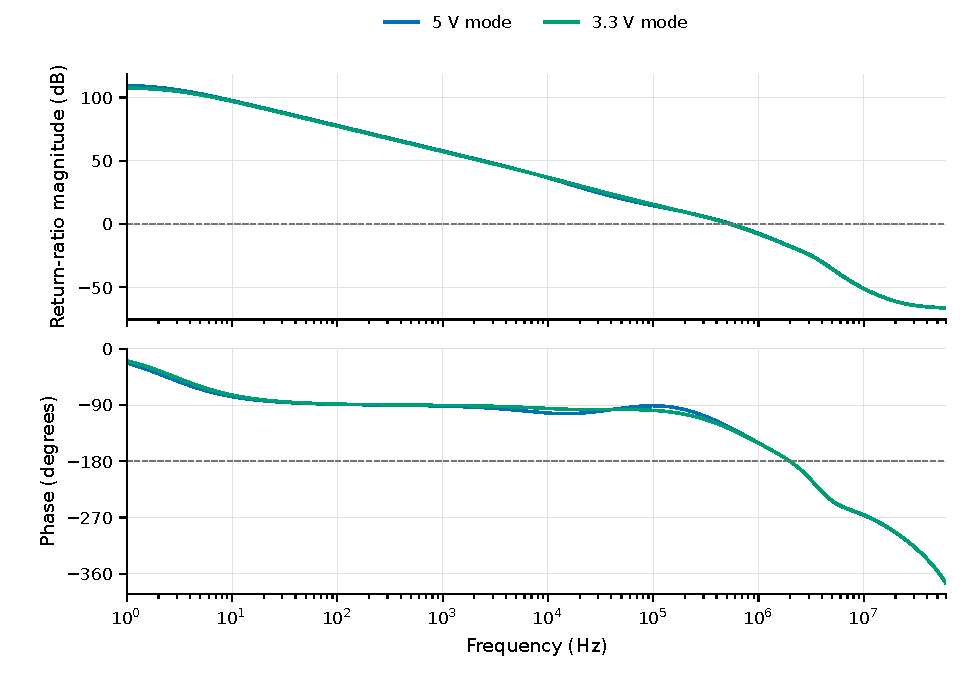
\includegraphics[width=0.95\textwidth]{SIM-09_core_loop.pdf}
\caption{Return ratio of the isolated regulation-loop bench (SIM-09),
with 5\,$\Omega$ and 3.3\,$\Omega$ loads, a 1\,$\mu$F output
capacitor and an external 1\,$\Omega$ series resistor,
with intrinsic capacitor ESR neglected. Auxiliary supply and control
biases are fixed. Dashed lines mark unity gain and \(-180^{\circ}\).}
\label{fig:regulation_loop_gain}
\end{figure*}

\begin{figure*}[t]
    \centering
    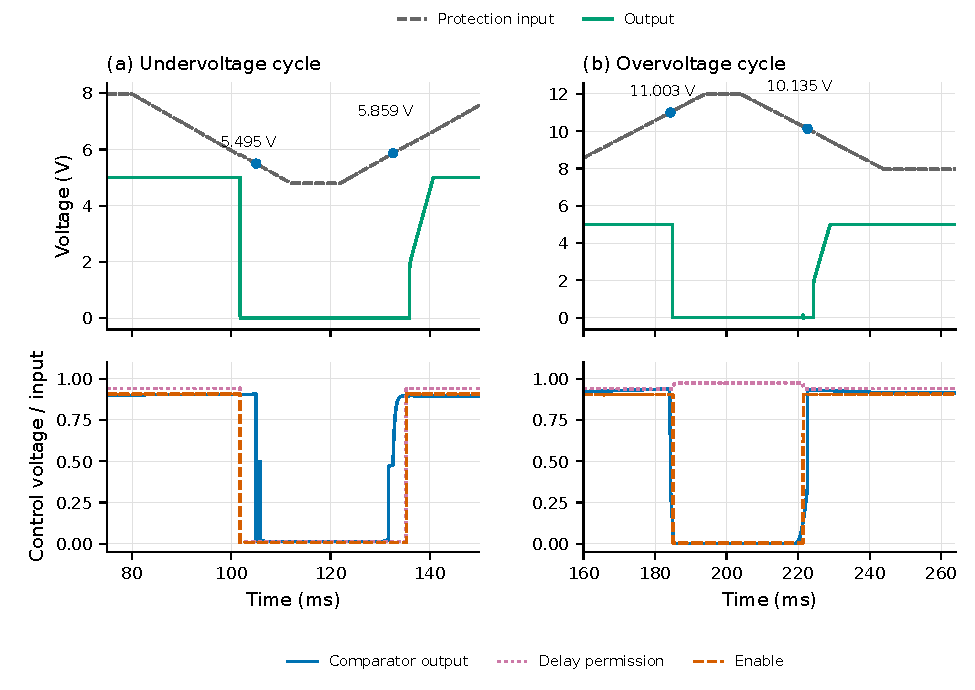
\includegraphics[width=0.95\textwidth]{SIM-07_calibrated_protection.pdf}
    \caption{Input-voltage protection in the calibrated complete circuit
    (SIM-07): \(5\,\mathrm{V}\) mode, \(5\,\Omega\) load,
    \(27\,^{\circ}\mathrm{C}\), and source ramps of
    \(0.1\,\mathrm{V/ms}\). Protection input denotes the supply
    after the test switch and polarity-protection MOSFET. Lower panels
    show control voltages divided by that supply. Markers identify
    comparator transitions, not combined-enable thresholds.}
    \label{fig:input_protection}
\end{figure*}

\subsection{Protection Characteristics}

Figure~\ref{fig:input_protection} verifies the UVLO and OVLO
hysteresis with the complete circuit (SIM-07). After startup at
\(8\,\mathrm{V}\), the source falls to \(4.8\,\mathrm{V}\),
rises to \(12\,\mathrm{V}\), and returns to \(8\,\mathrm{V}\).
Thresholds are extracted when each comparator output crosses
half of the local input supply. Table~\ref{tab:protection_characteristics}
reports the voltage at the protection-divider input at those instants,
for the stated ramp rate. The auxiliary reference remains available
during both input-fault holds.

The complete enable sequence also depends on the time-delay path.
During the falling-input test, this path removes enable at
approximately \(5.784\,\mathrm{V}\), before UVLO switches.
On recovery, UVLO grants permission first; combined enable returns
at approximately \(6.130\,\mathrm{V}\), after the delay condition
is satisfied. These are dynamic system events, distinct from the
comparator thresholds. Both undervoltage and overvoltage holds
disable the output, and regulation resumes after the permissions
are restored. The half-supply crossing is a measurement convention,
not the switching level of the discrete enable stage. This test covers the \(5\,\mathrm{V}\) configuration
and does not establish tolerance or temperature limits.

SIM-04 also checks the falling-input operating boundary in both
output modes, using 5\,$\Omega$ and 3.3\,$\Omega$ loads and the
same \(0.1\,\mathrm{V/ms}\) source ramp. The output crosses below
98\% of its nominal value at a source voltage of approximately
\(5.823\,\mathrm{V}\) in both modes, after the delay path removes
enable and before UVLO switches. Immediately before this sequence,
both outputs remain within 0.02\% of nominal. This is a dynamic
shutdown boundary, referenced to the source before the input switch;
it is neither an intrinsic dropout measurement nor a cold-start
minimum. A separate exploration sets RV10 to 100\,k$\Omega$ and
RV12 to 47\,k$\Omega$, within their available ranges, with
a 50\,$\Omega$ load in the 5\,V mode. Fixed-input
holds show approximately 100\,mV loss from the initial output
at a 4.95\,V source, while enable and the main reference
remain active. However, this condition involves approximately
147\,mA of pass-transistor base current. A terminal-power calculation
gives approximately 0.35\,W in Q3, exceeding the BC807's 250\,mW
rating on the manufacturer's standard footprint at 25\,$^\circ$C
\cite{nexperia_bc807_2022}. Continuous dropout testing therefore
requires verified thermal conditions. Pulsing only the external load
did not reduce driver dissipation in this dropout condition; the
measurement fixture must also establish a low-dissipation rest state.
These nominal-model results do not establish a hardware dropout
specification.




Figure~\ref{fig:current_limit} evaluates current limiting and recovery
with both calibrated output settings (SIM-08). A resistive overload
that would draw \(2\,\mathrm{A}\) at nominal voltage reduces the
output to approximately \(3.713\,\mathrm{V}\) in the 5\,V mode
and \(2.418\,\mathrm{V}\) in the 3.3\,V mode. A subsequent
\(50\,\mathrm{m}\Omega\) short produces a sustained load current
of approximately \(1.474\,\mathrm{A}\) in both modes.
Enable remains asserted throughout, and removing either fault
restores the selected output voltage without an enable cycle.

Current limiting is not instantaneous: the short-circuit transition
produces a brief current overshoot before the sustained limit is
established. The sense-resistor current also exhibits this transient;
it is not solely an output-capacitor discharge into the load.
Table~\ref{tab:protection_characteristics} reports averages over the
final \(10\,\mathrm{ms}\) of each fault hold, rather than transient
peaks. These nominal electrical simulations do not establish
continuous short-circuit thermal capability or safe operating area
of the pass transistor.

\begin{figure*}[t]
\centering
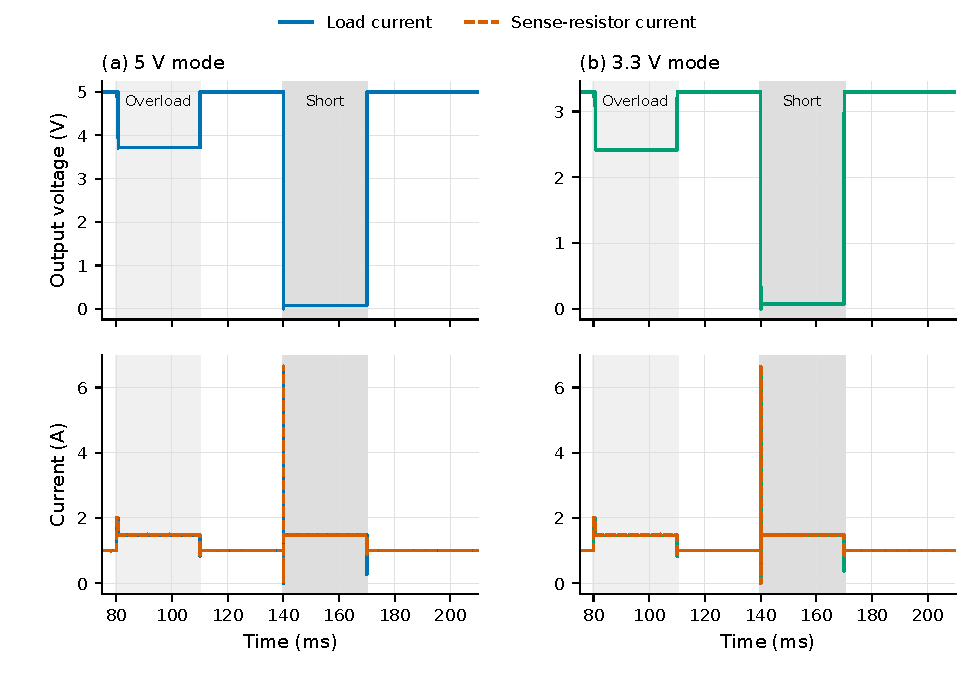
\includegraphics[width=0.95\textwidth]{SIM-08_calibrated_limit.pdf}
\caption{Overload, short-circuit and recovery response of the complete
calibrated regulator (SIM-08), with an 8\,V source at
27\,\textdegree C. Normal loads are 5\,$\Omega$ and 3.3\,$\Omega$.
Light shading marks overload (2.5\,$\Omega$ and 1.65\,$\Omega$);
darker shading marks a 50\,m$\Omega$ short in both modes.
Load conductance transitions last 10\,$\mu$s. Currents are shown
at the load and through the sense resistor toward the output.}
\label{fig:current_limit}
\end{figure*}

\begin{table*}[t]
\centering
\footnotesize
\setlength{\tabcolsep}{4pt}
\caption{Protection characteristics (LTspice, 27\,\textdegree C)}
\label{tab:protection_characteristics}
\begin{tabularx}{\textwidth}{@{}L{4.2cm}Xccc@{}}
\toprule
\textbf{Parameter} & \textbf{Conditions} & \textbf{Min} & \textbf{Typ} & \textbf{Max} \\
\midrule

UVLO rising threshold &
Protection input rising, comparator transition, SIM-07 &
-- & 5.859\,V & -- \\

UVLO falling threshold &
Protection input falling, comparator transition, SIM-07 &
-- & 5.495\,V & -- \\

UVLO hysteresis &
Difference between comparator thresholds, SIM-07 &
-- & 0.364\,V & -- \\

OVLO rising threshold &
Protection input rising, comparator transition, SIM-07 &
-- & 11.003\,V & -- \\

OVLO falling threshold &
Protection input falling, comparator transition, SIM-07 &
-- & 10.135\,V & -- \\

OVLO hysteresis &
Difference between comparator thresholds, SIM-07 &
-- & 0.868\,V & -- \\

Source voltage at 98\% output &
5\,V mode, falling 0.1\,V/ms, shutdown boundary, SIM-04 &
-- & 5.823\,V & -- \\

Source voltage at 98\% output &
3.3\,V mode, falling 0.1\,V/ms, shutdown boundary, SIM-04 &
-- & 5.823\,V & -- \\

Overload current &
5\,V mode, 8\,V source, 2.5\,$\Omega$ overload, SIM-08 &
-- & 1.485\,A & -- \\

Overload current &
3.3\,V mode, 8\,V source, 1.65\,$\Omega$ overload, SIM-08 &
-- & 1.465\,A & -- \\

Short-circuit current &
5\,V mode, 8\,V source, 50\,m$\Omega$ short, SIM-08 &
-- & 1.474\,A & -- \\

Short-circuit current &
3.3\,V mode, 8\,V source, 50\,m$\Omega$ short, SIM-08 &
-- & 1.474\,A & -- \\

Output voltage during short &
5\,V mode, 8\,V source, 50\,m$\Omega$ short, SIM-08 &
-- & 73.689\,mV & -- \\

Output voltage during short &
3.3\,V mode, 8\,V source, 50\,m$\Omega$ short, SIM-08 &
-- & 73.689\,mV & -- \\

\bottomrule
\end{tabularx}
\vspace{1mm}

\parbox{0.95\textwidth}{\footnotesize\emph{Note: UVLO/OVLO rows are dynamic comparator thresholds from SIM-07, distinct from the complete enable sequence. SIM-04 rows refer to the source before the input switch and do not measure intrinsic dropout. SIM-08 rows are time-weighted means over the final 10 ms of each fault hold; they exclude transient peaks and do not specify thermal capability. Hardware results may differ due to component tolerances, parasitics, temperature, and measurement uncertainty.}}
\end{table*}

\clearpage

% ======================================================================
% PCB PROTOTYPE
% ======================================================================
\raggedbottom
\section{PCB Prototype}

The simulated regulator was translated into a PCB layout to provide a practical implementation of the design. The board integrates the pass transistor, feedback network, reference stage, current-limit circuit, and input-voltage protection blocks described in the previous sections.

\begin{figure*}[t]
    \centering
    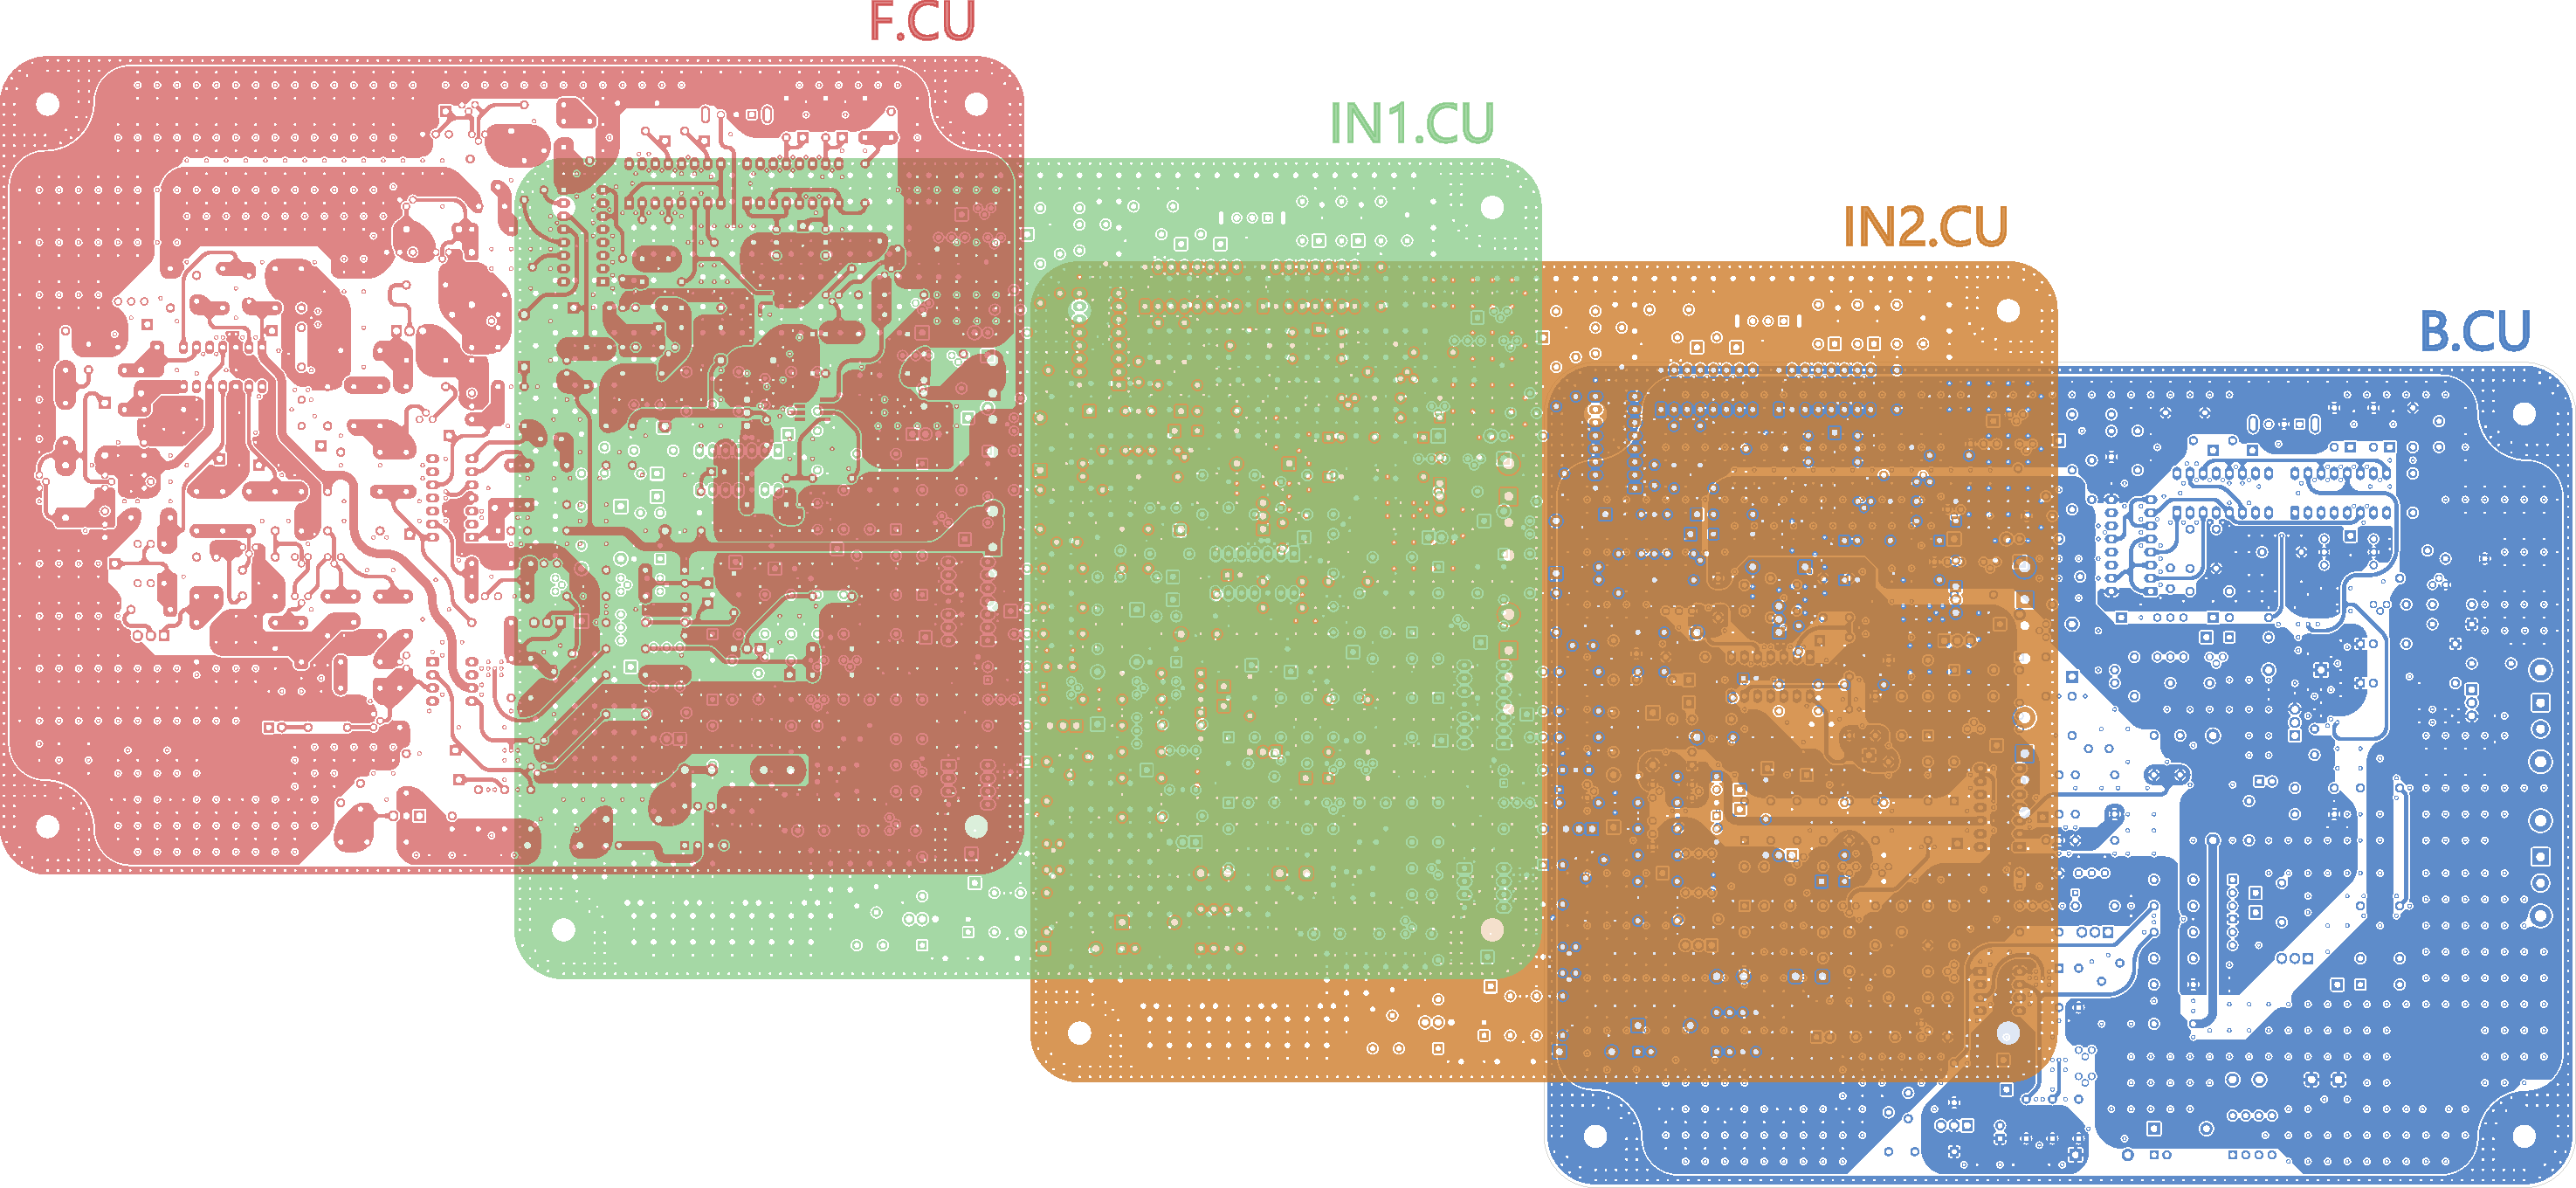
\includegraphics[width=0.95\textwidth]{coopper.pdf}
    \caption{Stacked PCB copper-layer view of the proposed linear regulator.}
    \label{fig:pcb_layout_stack}
\end{figure*}

The PCB was fabricated and assembled, and initial output checks confirmed operation in both the 5\,V and 3.3\,V settings. Exact readings, load conditions, and instrument details were not recorded in the present dataset, so these checks establish basic operation rather than quantified regulation accuracy.

The next measurements will characterize load regulation at a fixed input, followed by line regulation at a fixed load. Input and output voltages will be measured at the board terminals, with actual load current, instrument settings, and thermal conditions recorded. Calibration will remain unchanged within each sweep. Startup and shutdown waveforms will then be compared with the simulated sequence. Detailed procedures and original readings will be retained separately from the simulation results.

% ======================================================================
% CONCLUSION
% ======================================================================
\section{Conclusion}

This report presented a largely discrete linear regulator with selectable 5\,V and 3.3\,V outputs. The design uses a PNP pass transistor controlled by a feedback loop and includes current limiting, undervoltage lockout, and overvoltage lockout.

The calibrated simulations characterize line and load regulation, transient recovery, and protection behavior under stated nominal conditions. The regulation-loop analysis gives phase margins of approximately 52\,degrees at a load of approximately 1\,A with fixed auxiliary biases; it does not establish margins over the full operating range. The assembled PCB has passed initial checks of both output settings. Quantitative hardware measurements and thermal characterization remain necessary to assess practical performance against these simulation results.

% ======================================================================
% BIBLIOGRAPHY
% ======================================================================
\printbibliography

\end{document}
